% Se pre-carga la información del estudiante sólo para poder emplear el macro de
% selección de versión (digital o impresa)
% ===============================================================================
% El estudiante debe llenar sus datos en esta sección para que la plantilla los 
% auto-importe y genere automáticamente las páginas de portada y de firmas 
% autorizadas.
% ===============================================================================
% Datos del estudiante:
% -------------------------------------------------------------------------------
% Nombre completo
\def \nombreestudiante {Julio Andrés Avila}
% Carné
\def \uvgcarne {19285}
% Facultad
\def \uvgfacultad {Ingeniería}
% Carrera
\def \uvgcarrera {Ingeniería Mecatrónica}

% Datos del trabajo:
% -------------------------------------------------------------------------------
% Título completo
\def \titulotesis {Adaptación del sistema de drones Crazyswarm al ecosistema Robotat}
% Año de entrega
\def \anoentrega {2023}
% Asesor
\def \nombreasesor {Ing. Miguel Zea}

% Datos del tribunal examinador:
% -------------------------------------------------------------------------------
% Nombre del primer examinador
\def \nombreprimerex {MSc. Carlos Esquit}
% Nombre del segundo examinador
\def \nombresegundoex {Ing. Luis Pedro Montenegro}
% Año de aprobación
\def \anoaprobacion {2019}

% Capítulos pre-definidos
% -------------------------------------------------------------------------------
% Comentar las líneas de las secciones que desean omitirse, por defecto se 
% se incluyen todas.
\def \CAPprefacio {Prefacio}
\def \CAPantecedentes {Antecedentes}
\def \CAPalcance {Alcance}
\def \CAPanexos {Anexos}
%\def \CAPglosario {Glosario}

% Formato y estilo de la plantilla
% -------------------------------------------------------------------------------
% Modo impresión: Puede des-comentar la siguiente línea para generar un documento pdf sin la portada, para cuando se desee imprimir el documento para encuadernación
%\def \printver {Versión del documento para impresión}

% Portada: Puede cambiarse la imagen en la portada al cambiar el nombre del 
% archivo siguiente. NOTA: debe tener la suficiente resolución para cubrir el área
% designada
\def \imagenportada {plantilla/portadacit.jpg}

% Referencias: Puede des-comentar la siguiente línea para utilizar el formato de referencias APA
%\def \usarAPA {Usar formato APA}

% Párrafo: Puede comentar la siguiente línea si desea emplear un formato de 
% párrafo distinto al establecido por defecto
\def \parpordefecto {Formato de párrafo por defecto}

% Capítulos y secciones: Puede des-comentar la siguiente línea para establecer el
% formato de los capítulos y secciones bajo el estándar original de UVG para
% trabajos de graduación. Este incluye: capítulos con numeración romana, secciones
% con letras mayúsculas, sub-secciones con números y sub-sub-secciones con letras
% minúsculas
%\def \capsecuvg {Formato UVG para capítulos y secciones}

\ifdefined\printver
    \documentclass[11pt, letterpaper, twoside, openright]{report}
\else
    \documentclass[11pt, letterpaper]{report}
\fi

% Eliminar la opción de twoside y openright si se desea generar la versión
% digital del documento en lugar de la versión impresa
%\documentclass[11pt, letterpaper, twoside, openright]{report}
\usepackage[spanish, es-nodecimaldot, es-noquoting]{babel}
% cambiar a spanish, mexico si se quiere emplear tabla en lugar de cuadro
\selectlanguage{spanish}
\usepackage[utf8]{inputenc}
\usepackage[T1]{fontenc}

\title{Plantilla para Trabajos de Graduación IE-MT 2019v4}
\author{MSc. Miguel Zea}
\date{\today}

% Información del estudiante en el archivo datos_estudiante.tex
% ===============================================================================
% El estudiante debe llenar sus datos en esta sección para que la plantilla los 
% auto-importe y genere automáticamente las páginas de portada y de firmas 
% autorizadas.
% ===============================================================================
% Datos del estudiante:
% -------------------------------------------------------------------------------
% Nombre completo
\def \nombreestudiante {Julio Andrés Avila}
% Carné
\def \uvgcarne {19285}
% Facultad
\def \uvgfacultad {Ingeniería}
% Carrera
\def \uvgcarrera {Ingeniería Mecatrónica}

% Datos del trabajo:
% -------------------------------------------------------------------------------
% Título completo
\def \titulotesis {Adaptación del sistema de drones Crazyswarm al ecosistema Robotat}
% Año de entrega
\def \anoentrega {2023}
% Asesor
\def \nombreasesor {Ing. Miguel Zea}

% Datos del tribunal examinador:
% -------------------------------------------------------------------------------
% Nombre del primer examinador
\def \nombreprimerex {MSc. Carlos Esquit}
% Nombre del segundo examinador
\def \nombresegundoex {Ing. Luis Pedro Montenegro}
% Año de aprobación
\def \anoaprobacion {2019}

% Capítulos pre-definidos
% -------------------------------------------------------------------------------
% Comentar las líneas de las secciones que desean omitirse, por defecto se 
% se incluyen todas.
\def \CAPprefacio {Prefacio}
\def \CAPantecedentes {Antecedentes}
\def \CAPalcance {Alcance}
\def \CAPanexos {Anexos}
%\def \CAPglosario {Glosario}

% Formato y estilo de la plantilla
% -------------------------------------------------------------------------------
% Modo impresión: Puede des-comentar la siguiente línea para generar un documento pdf sin la portada, para cuando se desee imprimir el documento para encuadernación
%\def \printver {Versión del documento para impresión}

% Portada: Puede cambiarse la imagen en la portada al cambiar el nombre del 
% archivo siguiente. NOTA: debe tener la suficiente resolución para cubrir el área
% designada
\def \imagenportada {plantilla/portadacit.jpg}

% Referencias: Puede des-comentar la siguiente línea para utilizar el formato de referencias APA
%\def \usarAPA {Usar formato APA}

% Párrafo: Puede comentar la siguiente línea si desea emplear un formato de 
% párrafo distinto al establecido por defecto
\def \parpordefecto {Formato de párrafo por defecto}

% Capítulos y secciones: Puede des-comentar la siguiente línea para establecer el
% formato de los capítulos y secciones bajo el estándar original de UVG para
% trabajos de graduación. Este incluye: capítulos con numeración romana, secciones
% con letras mayúsculas, sub-secciones con números y sub-sub-secciones con letras
% minúsculas
%\def \capsecuvg {Formato UVG para capítulos y secciones}
% ================================================================================
% En este archivo se colocan opciones adicionales para modificar el formato de la
% plantilla, para emplearse en otros tipos de documentos que no sean trabajos de
% graduación. Si usted está trabajando su tesis, NO modifique este archivo
% ================================================================================
% Capítulos pre-definidos
% --------------------------------------------------------------------------------
% Comentar las líneas de las secciones que desean omitirse, por defecto se 
% se incluyen todas.
\def \CAPportada {Portada}
\def \CAPcaratula {Caratula}
\def \CAPfirmas {Hoja de firmas}
\def \CAPindice {Índice general}
\def \CAPfiguras {Listado de figuras}
\def \CAPcuadros {Listado de cuadros}
\def \CAPresumen {Resumen}
\def \CAPabstract {Resumen}
\def \CAPintroduccion {Introducción}
\def \CAPobjetivos {Objetivos}
\def \CAPjustificacion {Justificación}
\def \CAPmarcoteorico {Marco teórico}
\def \CAPconclusiones {Conclusiones}
\def \CAPrecomendaciones {Recomendaciones}
\def \CAPbibliografia {Bibliografía}

% ==============================================================================
% DEFINICIÓN DE PAQUETES
% ==============================================================================
\usepackage{xcolor}
\usepackage{amsfonts}
\usepackage{amsmath}
\usepackage{amssymb}
\usepackage{amsthm}
\usepackage{amsfonts}
\usepackage{mathtools}
\usepackage{graphicx}
\usepackage{xfrac}
\usepackage{float}
\usepackage{mathtools}
\usepackage[hypertexnames=false]{hyperref}
% \usepackage{bookmark}
\usepackage[font=small]{caption}
\usepackage{subcaption}
%\usepackage{csquotes}
\usepackage{xpatch}
\usepackage{emptypage}
\usepackage{hyphenat}
\usepackage{fancyhdr}
\usepackage[backend=biber, style=ieee]{biblatex}
\ifdefined\usarAPA 
    \usepackage[backend=biber, style=apa]{biblatex}
\fi
\addbibresource{m-bibliografia.bib}

\usepackage[percent]{overpic}

\usepackage{chngcntr}

\ifdefined\CAPglosario
	%\usepackage[toc]{glossaries}
	\usepackage[numberedsection]{glossaries}
	\makeglossaries
    \newglossaryentry{latex}
{
    name=latex,
    description={Es un lenguaje de marcado adecuado especialmente para la creación de documentos científicos}
} 
 
\newglossaryentry{formula}
{
    name=fórmula,
    description={Una expresión matemática} 
}
\fi

% ==============================================================================
% MÁRGENES Y FORMATO GENERALES
% ==============================================================================
\usepackage[top=1in, left=1.5in, right=1in, bottom=1in]{geometry}
%Options: Sonny, Lenny, Glenn, Conny, Rejne, Bjarne, Bjornstrup
\usepackage[Sonny]{fncychap}

% ==============================================================================
% DEFINICIONES DE LA PLANTILLA
% ==============================================================================
\graphicspath{ {figuras/} }
\definecolor{uvg-green}{RGB}{17,71,52}
\newcommand{\defaultparformat}[1]{
	{\setlength{\parskip}{2ex}
     \input{#1}}
}
\ifdefined\capsecuvg
	\renewcommand\thechapter{\Roman{chapter}}
    \renewcommand\thesection{\Alph{section}}
	\renewcommand\thesubsection{\arabic{subsection}}
    \renewcommand\thesubsubsection{\alph{subsubection}}
\fi
\counterwithout{figure}{chapter}
\counterwithout{table}{chapter}
\counterwithout{equation}{chapter}

\newcommand{\blankpage}{
\newpage
\thispagestyle{empty}
\mbox{}
\newpage
}
% ==============================================================================

% Comandos definidos por el usuario en el archivo comandos_usuario.tex
\input{2-paquetes_y_comandos_usuario}

% ==============================================================================
% CUERPO DEL TRABAJO
% ==============================================================================
\pagestyle{headings}
\begin{document}

% ==============================================================================
% PORTADA
% ==============================================================================
\ifdefined\printver
    \let\CAPportada\undefined
\fi 

\ifdefined\CAPportada
    \cleardoublepage\phantomsection
    % \pdfbookmark{Portada}{toc}
	\newgeometry{left=3cm, bottom=0in, top=1in, right=3cm}
	\pagecolor{uvg-green}
	\thispagestyle{empty}

	\color{white}
	\noindent \hrulefill \par
	\vspace{0.1in}
	\noindent \Huge \nohyphens{\titulotesis} \par
	\noindent \hrulefill \par
	\noindent
	\LARGE \nombreestudiante

	\begin{figure}[b!]
    	%\makebox[\textwidth]{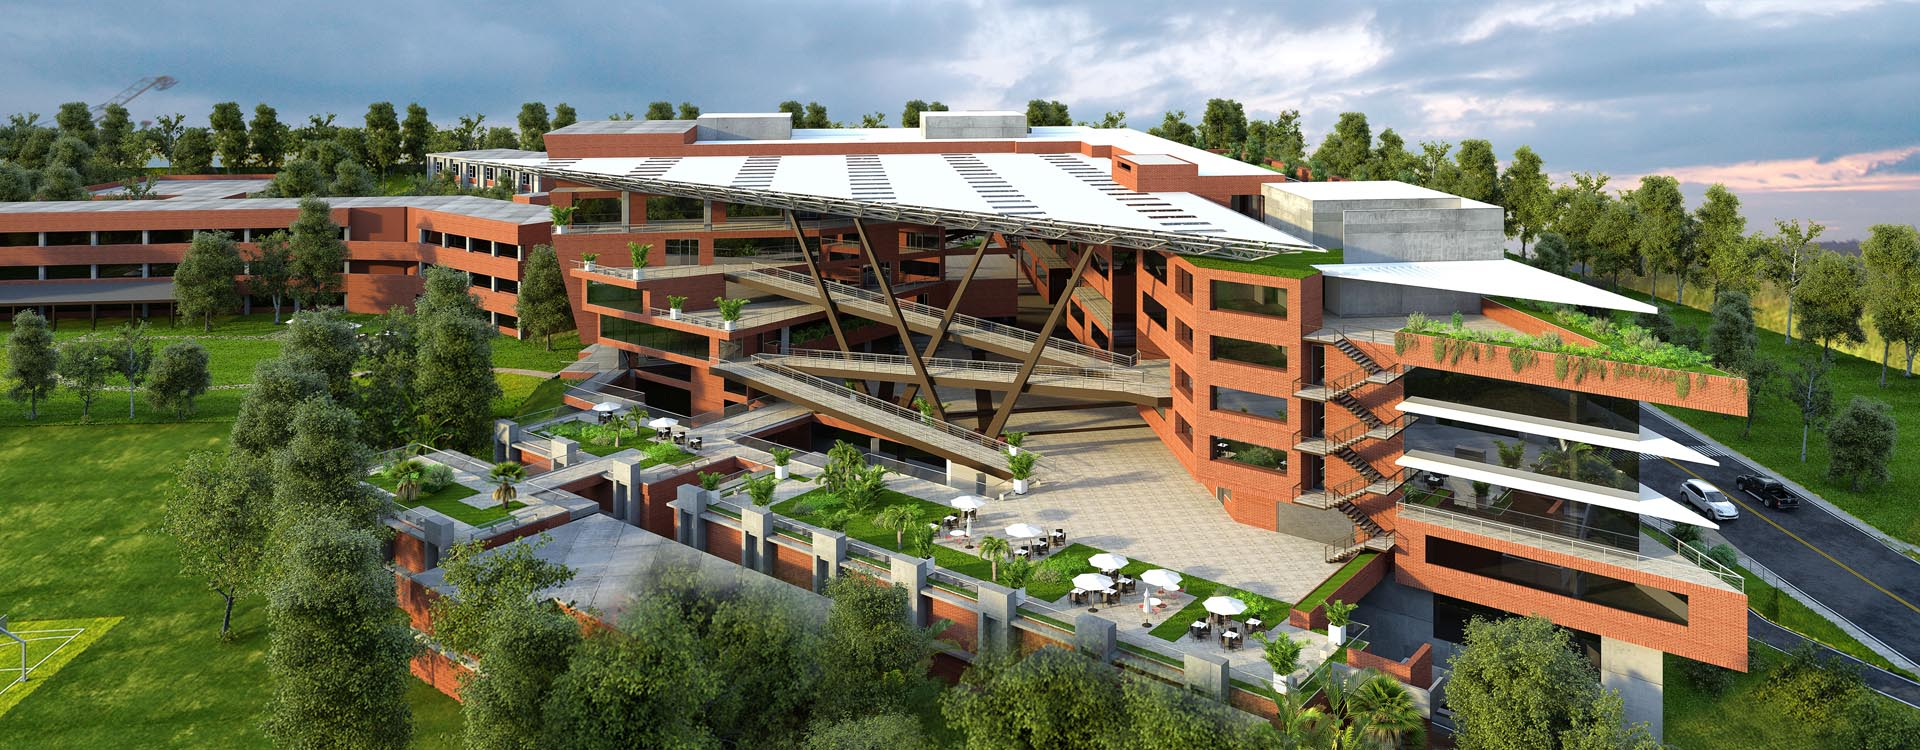
\includegraphics[height=13.25cm]{plantilla/portadacit.jpg}}
    	\makebox[\textwidth]{
    		\begin{overpic}[height=13.25cm]{\imagenportada}
     		\put(63,0){
\includegraphics[height=1.15in]{plantilla/fondologo_grande.png}}  
  			\put(64.5,2){
\includegraphics[height=0.55in]{plantilla/logoUVGblanco.eps}} 
        	\end{overpic}
    	}
    	%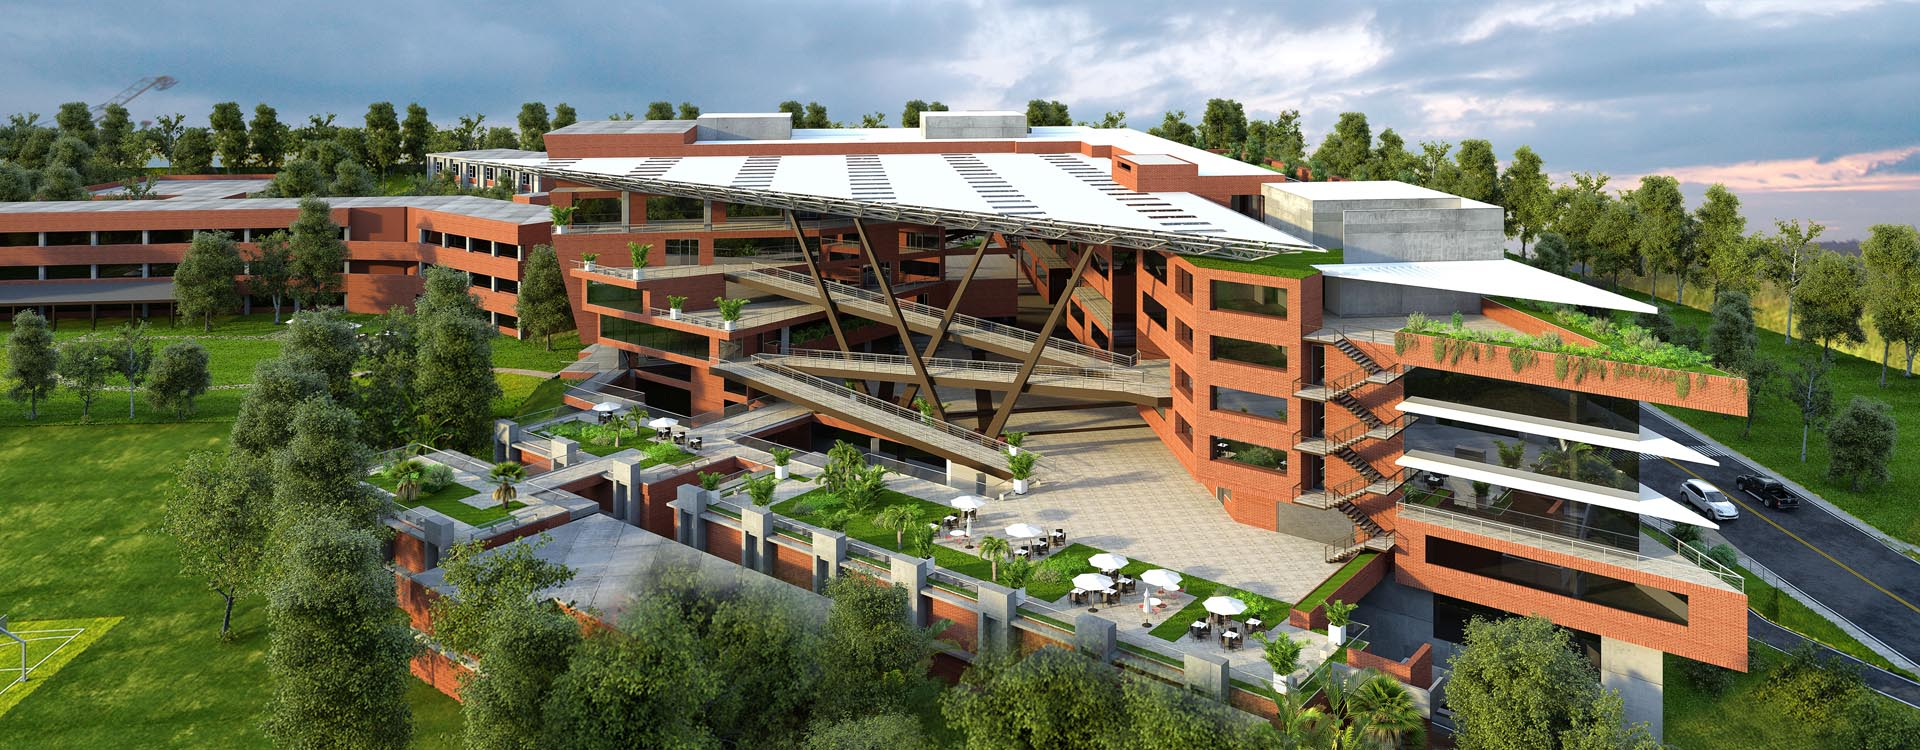
\includegraphics[height=13.25cm]{plantilla/portadacit.jpg}
	\end{figure}
	\restoregeometry
\fi

% ==============================================================================
% PRIMERAS PÁGINAS (Carátulas más hojas de guarda)
% ==============================================================================
\ifdefined\CAPcaratula
	\newpage
    \cleardoublepage\phantomsection
    % \pdfbookmark{Carátula}{toc}
	\pagecolor{white}
	\color{black}
	\setcounter{page}{1}
	\pagenumbering{roman}
	\thispagestyle{empty}
	\begin{center}
		\LARGE UNIVERSIDAD DEL VALLE DE GUATEMALA\\
		\LARGE Facultad de \uvgfacultad \\[0.75cm]
	\end{center}
	\begin{figure}[h]
		\begin{center}
		
\includegraphics[height=5.5 cm]{plantilla/escudoUVGnegro.eps}
		\vspace{0.5in}
		\end{center}
	\end{figure}
	\begin{center}
		\Large \textbf{\nohyphens{\titulotesis}} \\
		%\LARGE \textbf{\titulotesis} \\
		\vfill
		\Large \nohyphens{Trabajo de graduación presentado por \nombreestudiante \ para optar al grado académico de Licenciado en \uvgcarrera} \\
		\vfill
		\large Guatemala, \\
		\vspace{1em}
		\anoentrega
	\end{center}
    
    \ifdefined\printver	
	    \blankpage
	    \blankpage
	    
	    \newpage
	    \cleardoublepage\phantomsection
	    \pagecolor{white}
    	\color{black}
    	\setcounter{page}{1}
    	\pagenumbering{roman}
    	\thispagestyle{empty}
    	\begin{center}
    		\LARGE UNIVERSIDAD DEL VALLE DE GUATEMALA\\
    		\LARGE Facultad de \uvgfacultad \\[0.75cm]
    	\end{center}
    	\begin{figure}[h]
    		\begin{center}
    		
\includegraphics[height=5.5 cm]{plantilla/escudoUVGnegro.eps}
    		\vspace{0.5in}
    		\end{center}
    	\end{figure}
    	\begin{center}
    		\Large \textbf{\nohyphens{\titulotesis}} \\
    		%\LARGE \textbf{\titulotesis} \\
    		\vfill
    		\Large \nohyphens{Trabajo de graduación presentado por \nombreestudiante \ para optar al grado académico de Licenciado en \uvgcarrera} \\
    		\vfill
    		\large Guatemala, \\
    		\vspace{1em}
    		\anoentrega
    	\end{center}
    \fi
\fi

% ==============================================================================
% HOJA DE FIRMAS
% ==============================================================================
\ifdefined\CAPfirmas
	\newpage
	\cleardoublepage\phantomsection
	\thispagestyle{empty}
	\vspace*{0.5in}
	\large Vo.Bo.:\\[1cm]
	\begin{center}
		(f) \rule[1pt]{4 in}{1pt}\\
		\nombreasesor
	\end{center}
	\vspace{1in}

	Tribunal Examinador:\\[1cm]
	\begin{center}
		(f) \rule[1pt]{4 in}{1pt}\\
		\nombreasesor \\[1in]
		(f) \rule[1pt]{4 in}{1pt}\\
		\nombreprimerex \\[1in]
		(f) \rule[1pt]{4 in}{1pt}\\
		\nombresegundoex
	\end{center}
	\vspace{1in}

%	Fecha de aprobación: Guatemala, \rule[1pt]{0.5 in}{1pt} de \rule[1pt]{1 in}{1pt} de \anoaprobacion.
    Fecha de aprobación: Guatemala, \diaaprobacion de \mesaprobacion de \anoaprobacion.
	\normalsize
\fi

% Comentar para formato estilo libro en la numeración de páginas (NO 
% compatible con la guía UVG 2019)
\pagestyle{plain}
% ==============================================================================
% CONTENIDO DEL TRABAJO
% ==============================================================================
% PREFACIO
% ------------------------------------------------------------------------------
\ifdefined\CAPprefacio
	\newpage
	\cleardoublepage\phantomsection
    \chapter*{Prefacio}
    \ifdefined\parpordefecto
    	\defaultparformat{a-prefacio}
    \else
    	Lorem ipsum dolor sit amet, consectetur adipiscing elit. Cras vitae eleifend ipsum, ut mattis nunc. Pellentesque ac hendrerit lacus. Cras sollicitudin eget sem nec luctus. Vivamus aliquet lorem id elit venenatis pellentesque. Nam id orci iaculis, rutrum ipsum vel, porttitor magna. Etiam molestie vel elit sed suscipit. Proin dui risus, scelerisque porttitor cursus ac, tempor eget turpis. Aliquam ultricies congue ligula ac ornare. Duis id purus eu ex pharetra feugiat. Vivamus ac orci arcu. Nulla id diam quis erat rhoncus hendrerit. Class aptent taciti sociosqu ad litora torquent per conubia nostra, per inceptos himenaeos. Sed vulputate, metus vel efficitur fringilla, orci ex ultricies augue, sit amet rhoncus ex purus ut massa. Nam pharetra ipsum consequat est blandit, sed commodo nunc scelerisque. Maecenas ut suscipit libero. Sed vel euismod tellus.

Proin elit tellus, finibus et metus et, vestibulum ullamcorper est. Nulla viverra nisl id libero sodales, a porttitor est congue. Maecenas semper, felis ut rhoncus cursus, leo magna convallis ligula, at vehicula neque quam at ipsum. Integer commodo mattis eros sit amet tristique. Cras eu maximus arcu. Morbi condimentum dignissim enim non hendrerit. Sed molestie erat sit amet porttitor sagittis. Maecenas porttitor tincidunt erat, ac lacinia lacus sodales faucibus. Integer nec laoreet massa. Proin a arcu lorem. Donec at tincidunt arcu, et sodales neque. Morbi rhoncus, ligula porta lobortis faucibus, magna diam aliquet felis, nec ultrices metus turpis et libero. Integer efficitur erat dolor, quis iaculis metus dignissim eu.
    \fi
    \addcontentsline{toc}{chapter}{Prefacio}
\fi

% ÍNDICE GENERAL
% ------------------------------------------------------------------------------
\ifdefined\CAPindice
	\newpage
    \cleardoublepage\phantomsection
	\renewcommand{\contentsname}{Índice}
    %\phantomsection
    \pdfbookmark{\contentsname}{toc}
    %\pdfbookmark{Índice}{toc}
	\tableofcontents
\fi

% LISTADO DE FIGURAS
% ------------------------------------------------------------------------------
\ifdefined\CAPfiguras
	\newpage
    \cleardoublepage\phantomsection
	\renewcommand{\listfigurename}{Lista de figuras}
	\listoffigures
	\addcontentsline{toc}{chapter}{Lista de figuras}
\fi

% LISTADO DE CUADROS
% ------------------------------------------------------------------------------
\ifdefined\CAPcuadros
	\newpage
    \cleardoublepage\phantomsection
	\renewcommand{\listtablename}{Lista de cuadros}
	\listoftables
	\addcontentsline{toc}{chapter}{Lista de cuadros}
\fi

% RESUMEN
% ------------------------------------------------------------------------------
\ifdefined\CAPresumen
	\newpage
    \cleardoublepage\phantomsection
	\chapter*{Resumen}
	\ifdefined\parpordefecto
		\defaultparformat{b-resumen}
	\else
		La Universidad del Valle de Guatemala cuenta con un laboratorio de Robótica llamado Robotat,  el cual cuenta con un sistema de captura de movimiento y se trabajan líneas de investigación relacionadas con sistemas de control y robótica, además de ser el espacio donde se realizan las prácticas de laboratorio de los cursos de robótica. Está diseñado para realizar pruebas con agentes autónomos, entre ellos robots humanoides, robots móviles con ruedas, brazos robóticos y drones.

Entre los drones a utilizar se encuentran los drones Crazyflie 2.1, los cuales son de tamaño pequeño y pueden emplearse en conjunto para controlar enjambres de drones. Se planea realizar este control mediante el sistema Crazyswarm, el cual funciona a trvés de ROS2 en Linux. Con el objetivo de que este sistema de drones pueda utilizarse en prácticas de laboratorio y otras líneas de investigación en la Universidad, se adaptará la infraestructura de este sistema al ecosistema Robotat a través de los paquetes y funciones de ROS2. Esto podrá realizarse mediante la obtención de paquetes de información generados por los algoritmos de control y el sistema de captura de movimiento del Robotat, logrando una integración entre los drones y el laboratorio.
	\fi
	\addcontentsline{toc}{chapter}{Resumen}
\fi

% ABSTRACT
% ------------------------------------------------------------------------------
\ifdefined\CAPabstract
	\newpage
    \cleardoublepage\phantomsection
	\chapter*{Abstract}
	\ifdefined\parpordefecto
		\defaultparformat{c-abstract}
	\else
		This is an abstract of the study developed under the
	\fi
	\addcontentsline{toc}{chapter}{Abstract}
\fi

% INTRODUCCIÓN
% ------------------------------------------------------------------------------
\ifdefined\CAPintroduccion
	\newpage
	\cleardoublepage
	\pagenumbering{arabic}
	\setcounter{page}{1}
	\chapter{Introducción}
	\ifdefined\parpordefecto
		\defaultparformat{d-introduccion}
	\else
		Lorem ipsum dolor sit amet, consectetur adipiscing elit. Quisque eget consequat risus. Praesent a quam lacinia, consequat eros id, auctor tellus. Phasellus a dapibus arcu, vitae luctus leo. Aliquam erat volutpat. Suspendisse ac velit quam. Nullam risus nibh, lobortis vehicula elit non, pellentesque volutpat odio. Donec feugiat porta sapien gravida interdum. Cras odio nunc, lobortis sed pellentesque imperdiet, facilisis eu quam. Praesent pharetra, orci at tincidunt lacinia, neque nulla ornare lacus, ut malesuada elit risus non mi. Fusce pellentesque vitae sapien sed mollis. Curabitur viverra at nulla vitae porta. In et mauris lorem.

Vestibulum faucibus fringilla justo, eget facilisis elit convallis sit amet. Morbi nisi metus, hendrerit quis pellentesque non, faucibus at leo. Proin consectetur, est vel facilisis facilisis, arcu felis vestibulum quam, et fringilla metus neque at enim. Nunc justo mauris, egestas quis maximus eget, viverra vehicula nunc. Fusce eu nulla elementum, condimentum diam at, aliquam leo. Nullam sed sodales enim, eu imperdiet risus. Aliquam ornare augue leo, fringilla mattis nunc facilisis eget. Nam faucibus, libero a aliquet fermentum, magna arcu ultrices lacus, a placerat tortor turpis ut purus.

Integer eget ligula non metus egestas rutrum sit amet ut tellus. Aliquam vel convallis est, eu sodales leo. Proin consequat nisi at nunc malesuada gravida. Aliquam erat volutpat. Aliquam finibus interdum dignissim. Etiam feugiat hendrerit nisl, hendrerit feugiat ex malesuada in. Cras tempus eget arcu vitae congue. Ut non tristique mauris. Vivamus in mattis ipsum. Cras bibendum, enim bibendum commodo accumsan, ligula nulla porttitor ex, et pharetra eros nisl eget ex. Morbi at semper arcu. Curabitur massa sem, maximus id metus ut, molestie tempus quam. Vivamus dictum nunc vitae elit malesuada convallis. Donec ac semper turpis, non scelerisque justo. In congue risus id vulputate gravida. Nam ut mattis sapien.
	\fi
\fi

% ANTECEDENTES
% ------------------------------------------------------------------------------
\ifdefined\CAPantecedentes
	\newpage
	\chapter{Antecedentes}
	\ifdefined\parpordefecto
    	\defaultparformat{e-antecedentes}
    \else
    	Los drones Crazyflie se han utilizado en líneas de investigación relacionadas con sistemas de control y robótica de enjambre debido a su extensa documentación y versatilidad para desarrollo de algoritmos. Para poder realizar un control eficiente de múltiples agentes, es necesario implementar un sistema que sea capaz de obtener y procesar información acerca del comportamiento de los agentes en tiempo real.
\subsubsection*{Crazyflie 2.1}

Los drones a trabajar durante esta línea de investigación son los Crazyflies 2.1, los cuales son cuadricópteros de tamaño pequeño, que pueden ser controlados mediante un sistema de control de enjambre llamado Crazyswarm, el cual es utilizado mediante ROS en Ubuntu. 

Anteriormente, se trabajó con estos drones en una línea de investigación pero no en forma de enjambre, sino con un drone únicamente. Se desarrollaron herramientas para el uso individual de estos drones. En primer lugar, se comprobó la compatibilidad de comunicación entre un drone y Python para el análisis de datos, estos se guardan en bruto y se recomendó graficarlos posteriormente mediante Matlab. Se desarrolló una interfaz gráfica para prácticas de laboratorio, en la cual, se pudo observar el comportamiento del drone ante las propiedades de control determinadas, en este caso, un controlador PID y sus respectivas constantes. Cabe destacar que para poder hacer esta herramienta fue necesario plantear un modelo matemático a través del identificador de sistemas de Matlab. Como resultado de estas herramientas, se llegaron a planificar 2 prácticas de laboratorio para los cursos de Sistemas de Control. \cite{Sanabria2022_tesis}

\subsubsection*{Ecosistema Robotat}

El objetivo principal es utilizar este enjambre de drones en el ecosistema Robotat, el cual es un entorno tecnológico ubicado en el laboratorio de Robótica CIT-116 de la Universidad del Valle de Guatemala. \cite{Camilo2022_tesis}Se implementó un sistema de captura de movimiento mediante un set de 6 cámaras de la marca OptiTrack, las cuales están conectadas a un switch que se comunica con una computadora mediante UDP, también fue implementado un protocolo MQTT para establecer una comunicación Wi-Fi. La información recopilada es procesada mediante un algoritmo de Python y luego es enviada a un router que genera una red Wi-Fi local a la cual es posible conectar diferentes dispositivos y obtener datos como posiciones lineales y angulares. Las cámaras están colocadas de tal forma que rodean una tarima hecha de concreto y acero, como se muestra en la Figura \ref{fig:Robotat}. 

\begin{figure}[t]
    \centering
    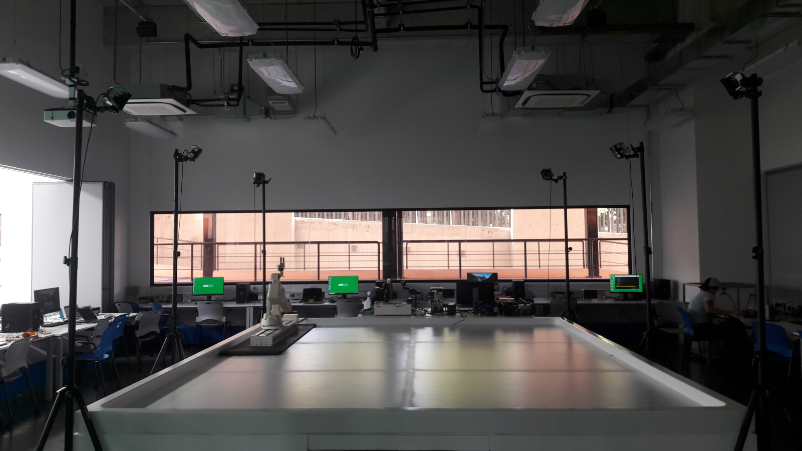
\includegraphics[width=0.5\textwidth]{figuras/Robotat.png}
    \caption{Ecosistema Robotat.}
    \cite{Camilo2022_tesis}
    \label{fig:Robotat}
\end{figure}

\subsubsection{Crazyswarm y ROS2}

ROS es un sistema operativo para sistemas robóticos, el cual provee funciones especiales que facilitan el análisis y control en proyectos de robótica. Este suele trabajarse en sistemas basados en Linux como Ubuntu. A través de ROS2 puede trabajarse Crazyswarm, el cual es un sistema para controlar enjambres de drones Crazyflie 2.1, además se cuenta con un cliente llamado Bitcraze, el cual está basado en Python y permite la comunicación entre el servidor y los drones mediante telecomunicación por radiofrecuencia, este es un sistema independiente de ROS. El entorno Crazyswarm está siendo reemplazado por la versión 2, a la cual se le han estado trabajando mejoras. 

El posicionamiento de los drones se ha realizado de múltiples maneras en distintas líneas de investigación, entre la documentación oficial de Crazyswarm puede encontrarse información sobre pruebas realizadas en sistemas de captura de movimiento, tales como OptiTrack. Para poder realizar experimentos con OptiTrack es necesario implementar un módulo con marcadores reflectivos y este debe estar diseñado a la medida para que el drone pueda ser detectado por las cámaras. Otros métodos utilizados para el posicionamiento de drones es mediante un dispositivo Kinect de la marca Microsoft, utilizado en consolas Xbox. \cite{Crazyswarm}


    \fi  
\fi

% JUSTIFICACIÓN
% ------------------------------------------------------------------------------
\ifdefined\CAPjustificacion
	\newpage
	\chapter{Justificación}
	\ifdefined\parpordefecto
		\defaultparformat{f-justificacion}
	\else
		Los drones son dispositivos que han ganado popularidad en los últimos años por una característica especial, ya que al modelarlos como un sistema dinámico se presenta una dinámica no lineal, pero pueden ser controlados de forma satisfactoria con un controlador lineal, siendo este un control relativamente sencillo. Esto convierte a los drones en un excelente método de aprendizaje para diseñar y analizar modelos y algoritmos de control. Debido a esto, trabajar físicamente con un drone o inclusive, con un conjunto de estos, es una alternativa para poner en práctica los aprendizajes adquiridos a lo largo de una carrera universitaria relacionada con electrónica y para realizar investigación relaciona con sistemas de control clásico, moderno y robótica de enjambre. Para poder realizar esto, es necesario contar con un medio que le provea a los algoritmos de control la información necesaria para trabajar, incluyendo, pero no limitándose, a las posiciones espaciales y orientaciones de los respectivos drones. Debido a que se cuenta con un entorno que es capaz de capturar esta información física, el camino a tomar es la creación de un intermediario que permita la comunicación entre el sistema de captura y los algoritmos de control para drones.

El ecosistema Robotat fue creado como un entorno tecnológico que sirviera como un lugar de aprendizaje de sistemas robóticos y para desarrollar lineas de investigación relacionadas con sistemas de control y robótica. Para culminar el desarrollo de este entorno, es necesario integrar a todos los agentes autónomos que formarán parte de él, siendo los drones Crazyflie una parte importante del ecosistema. 
	\fi
\fi

% OBJETIVOS
% ------------------------------------------------------------------------------
\ifdefined\CAPobjetivos
	\newpage
	\chapter{Objetivos}
	\ifdefined\parpordefecto
		\defaultparformat{g-objetivos}
	\else
		\subsection*{Objetivo general}
Adaptar el sistema de control de drones Crazyswarm al ecosistema Robotat mediante ROS2 y sus respectivos paquetes y funciones.

\subsection*{Objetivos específicos}
\begin{itemize}
\item Emplear la información recibida por las cámaras de captura OptiTrack en el ecosistema Robotat para definir algoritmos de control del sistema de drones.
\item Crear algoritmos que conviertan información de origen TCP/UDP a radio frecuencia para establecer una comunicación directa con Crazyswarm.
\item Levantar la infraestructura de Crazyswarm y desarrollar pruebas iniciales de vuelo.
\end{itemize}
	\fi
\fi

% ALCANCE
% ------------------------------------------------------------------------------
\ifdefined\CAPalcance
	\newpage
	\chapter{Alcance}
	\ifdefined\parpordefecto
    	\defaultparformat{h-alcance}
    \else
    	Podemos usar \Gls{latex} para escribir de forma ordenada una \gls{formula} matemática. 
    \fi 
\fi

% MARCO TEÓRICO
% ------------------------------------------------------------------------------
\ifdefined\CAPmarcoteorico
	\newpage
	\chapter{Marco teórico}
	\ifdefined\parpordefecto
		\defaultparformat{i-marco_teorico}
	\else
		\subsection*{Crazyflie}
Los drones Crazyflie son micro drones de dimensiones significativamente pequeñas (92x92x29 mm) y una masa de 27 g, cuentan con cuatro motores con un diseño simétrico. 

El control directo de estos drones se realiza mediante radio frecuencia, específicamente a una frecuencia de 2.4 GHz, la cual pertenece a la banda de radios ISM. Cuenta con un amplificador de radio de 20 dB, con el cual se puede trabajar en un radio de hasta 1 km. Entre sus características eléctricas, se encuentra un microcontrolador STM32F405, el cual corre a 168 MHz. Este microcontrolador presenta una gran ventaja al trabajar a una velocidad alta ya que se puede garantizar un procesamiento de señales y una ejecución de algoritmos eficientes. Cuenta con un cargador LiPo con modos de 100 mA hasta 980 mA, el tiempo de vuelo estimado con la batería cargada es de 7 minutos, con un tiempo de carga de 40 minutos. Según Bitcraze, es recomendado que cualquier carga adicional que soporte el drone no supere los 15 g. \ref{fig:Crazyflie 2.1}

\begin{figure}[t]
    \centering
    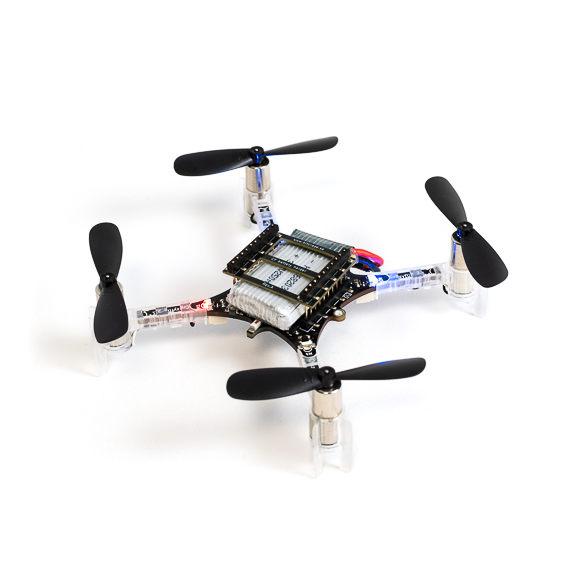
\includegraphics[width=0.5\textwidth]{figuras/crazyflie_2.1_585px.jpg}
    \caption{Crazyflie 2.1.}
    \cite{Crazyflie_2.1}
    \label{fig:Crazyflie 2.1}
\end{figure}

\subsection*{Control y estimación de estado}
La IMU del Crazyflie 2.1 cuenta con un acelerómetro/giroscopio de 3 de ejes BMI080 y un sensor de presión BMP388. El control del drone se basa en un modelo de sistema dinámico. El modelado de sistemas dinámicos es utilizado en sistemas de control y robótica para diseñar un controlador basado en la naturaleza del sistema, obteniendo un modelo matemático de este. Las variables de estado son valores determinados de un sistema dinámico, el cual puede ser un sistema físico, mecánico, eléctrico, etc. En el caso de un drone cuadricóptero, las variables de estado son los ángulos de rotación alrededor de sus ejes (\emph{roll}, \emph{pitch}, \emph{yaw}), su posición en el espacio y cómo estas variables cambian en el tiempo (sus derivadas). Para el caso de Crazyflie, las variables fundamentales a controlar son dichos ángulos y la altitud de este. Se utilizan estimaciones de estado para convertir las señales de los sensores en variables de estado y así poder realizar el respectivo control.  

Debido a que se utilizan métodos externos para determinar el estado de los drones, siendo un sistema de captura de movimiento para este caso, es necesario combinar las mediciones internas del drone con las externas por lo que se utiliza el filtro de Kalman como observador de estado. Los observadores de estado son algoritmos que utilizan el modelo matemático del sistema y mediciones del mismo para dar una estimación de las variables de estado. El filtro de Kalman es un observador de estado que toma en cuenta el ruido generado por perturbaciones en los actuadores o sensores del sistema, modelándolos como ruido blanco no correlacionado. Los drones Crazyflie utilizan un filtro de Kalman extendido como un filtro recursivo que estima el estado actual del drone basado en las mediciones internas y externas y el modelo matemático del mismo. \cite{Kalman}

El control de los drones se realiza mediante una arquitectura de controladores PID en cascada, donde la entrada de control es la posición y la velocidad esperada, que luego determina ángulos de \emph{pitch} y \emph{roll} deseados, seguido de una velocidad angular y finalmente determina el \emph{thrust} de los motores. \ref{fig:PID}
\begin{figure}[t]
    \centering
    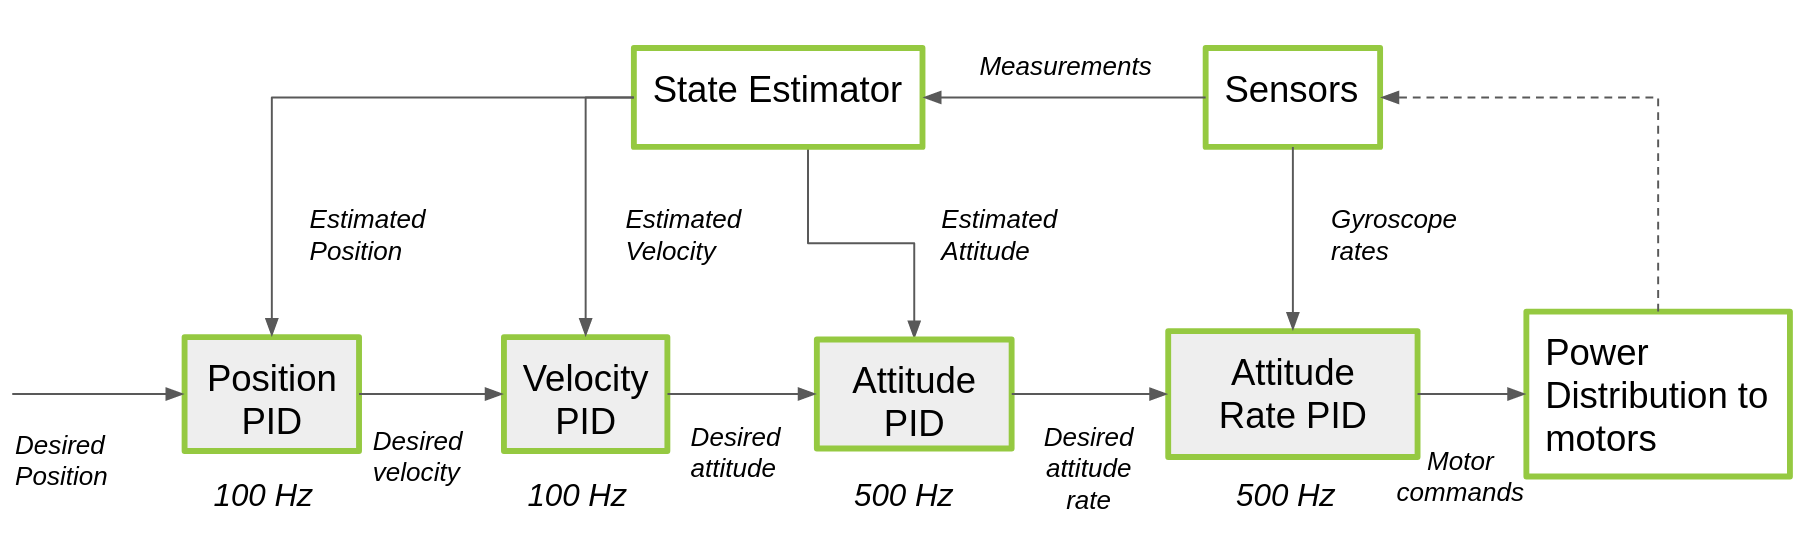
\includegraphics[width=0.8\textwidth]{figuras/cascaded_pid_controller.png}
    \caption{Arquitectura de Control.}
    \cite{Kalman}
    \label{fig:PID}
\end{figure}

\subsection*{Sistemas de radio frecuencia}
La comunicación por Radio Frecuencia (RF) es una tecnología para las telecomunicaciones que se da por un dispositivo que crea ondas electromagnéticas a altas frecuencias, donde las ondas se propagan en el espacio alcanzando a otro dispositivo receptor que procese la información a la misma frecuencia. Según la frecuencia de las ondas, las comunicación puede clasificarse en \begin{itemize}
    \item VLF: 3 kHz - 30 kHz
    \item LF: 30 kHz - 300 kHz
    \item HG: 3 MHz - 30 MHz
    \item VHF: 30 MHz - 300 MHz
    \item UHF: 300 MHz - 3 GHz
    \item SHF: 3 GHz - 30 GHz
    \item EHF: 30 GHz - 300 GHz
\end{itemize}
Las antenas convierten la información digital en señales eléctricas y luego en ondas electromagnéticas, o viceversa en el caso de la recepción de información. La ventaja que presenta este tipo de comunicación es que el dispositivo que procese tanto la información enviada como recibida puede ser un microcontrolador, siempre que este tenga la capacidad de conectarse a una antena y funcione a una frecuencia lo suficientemente alta como para procesar la señal de radio y digitalizar la información.

\subsection*{Protocolos de redes}
Para crear una comunicación eficiente se debe trabajar en conjunto con protocolos de comunicación por redes, como TCP, el cual divide la información en paquetes y garantiza que estos lleguen correctamente a su destino. El protocolo TCP, que significa \emph{Transmission Control Protocol}, es un protocolo de 3 vías donde primero se envía una solicitud inicial (\emph{SYN}) desde el origen, luego el destino envía un paquete de confirmación (\emph{SYN-ACK)} y finalmente el origen envía un último paquete (\emph{ACK}) seguido de la información a transmitir. Este trabaja en conjunto con el protocolo IP, el cual se encarga unicamente asegurar una conexión entre el servidor de origen y destino mediante el sistema de direcciones de Internet.

El \emph{User Datagram Protocol}, o UDP, es un protocolo de comunicación de Internet que, a diferencia del TCP, permite una comunicación rápida al no requerir que se establezca formalmente una conexión antes de iniciar con las transmisión de datos, sin embargo, esto también provoca que los paquetes puedan perderse en tránsito. \cite{UDP}

\subsection*{Formato JSON}
Para la estructura de los datos transferidos entre los distintos medios de comunicación, puede implementarse el formato \emph{JavaScript Object Notation} (JSON), el cual es ligero computacionalmente y de fácil lectura y escritura. Adicionalmente, puede aplicarse a otros lenguajes de programación, como C, C++, Python, etc.

\subsection*{Sistemas de captura de movimiento}

La captura de movimiento es una tecnología que ha ganado popularidad los últimos años al emplearse en aplicaciones como animación, videojuegos o investigación de sistemas mecánicos. Este proceso se da mediante cámaras de luz infrarroja, la cual se apunta hacia el sistema o conjunto de sistemas a capturar, los cuales deben contar con algún material que refleje la luz. En el caso particular de las cámaras de la marca Optitrack, las cuales son utilizadas en el Robotat en la Universidad del Valle de Guatemala (figura \ref{fig:camara}), cuentan con un set de emisores de luz infrarroja y utiliza pequeñas bolas cubiertas de material reflejante, conocidas como marcadores. Este tipo de captura de movimiento es conocido como óptica pasiva, ya que los marcadores reflejan la luz en lugar de generarla. \cite{Camilo2022_tesis}

\begin{figure}[t]
    \centering
    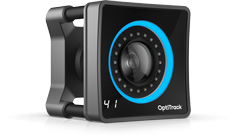
\includegraphics[width=0.5\textwidth]{figuras/primeX41-perspective-235.png}
    \caption{Cámara de captura OptiTrack.}
    \cite{OptiTrack_Primex-40}
    \label{fig:camara}
\end{figure}

Los marcadores pueden usarse de forma individual para rastrear unicamente posiciones, o bien pueden trabajarse en grupos de 3 con una forma en específico para analizar también la orientación de los cuerpos.

\subsection*{Ecosistema Robotat}

Para transferir los datos obtenidos por el sistema de captura en el Robotat, las cámaras OptiTrack están conectadas a un Switch que se comunica con un servidor mediante un protocolo UDP. La información es procesada  y enviada mediante un servidor de Python que posteriormente se comunica con un router Wi-Fi, el cual permite la comunicación entre dispositivos externos y agentes autónomos en el Robotat. Esta comunicación entre el router y los dispositivos se logra mediante un protocolo TCP, de esta forma puede accederse directamente a la información mediante la de composición de un documento de tipo JSON.

\subsection*{Cliente de Crazyflie y ROS2}

ROS funciona con nodos, creando un servidor de Crazyflie que establece la comunicación directa entre los drones y la interfaz utilizada, que en este caso es ROS2 junto con la API de Python como se ve en la Figura \ref{fig:nodos}.

El control de los drones se divide en cuatro capas independientes. La capa física transmite los paquetes de información desde y hacia el drone, donde puede implementarse una antena de radiofrecuencia para esto. El \emph{link} implementa los canales para los paquetes, abstrayendo el medio físico e implementando un canal de transmisión y otro de recepción entre el Crazyflie. El CRTP, acrónimo de \emph{Crazy Realtime Protocol}, implementa la información del puerto y el canal para crear la ruta del paquete a varios subsistemas. Finalmente, los subsistemas implementan las funcionalidades del Crazyflie que pueden ser controladas, habiendo sólo un puerto por subsistema.

\begin{figure}[t]
    \centering
    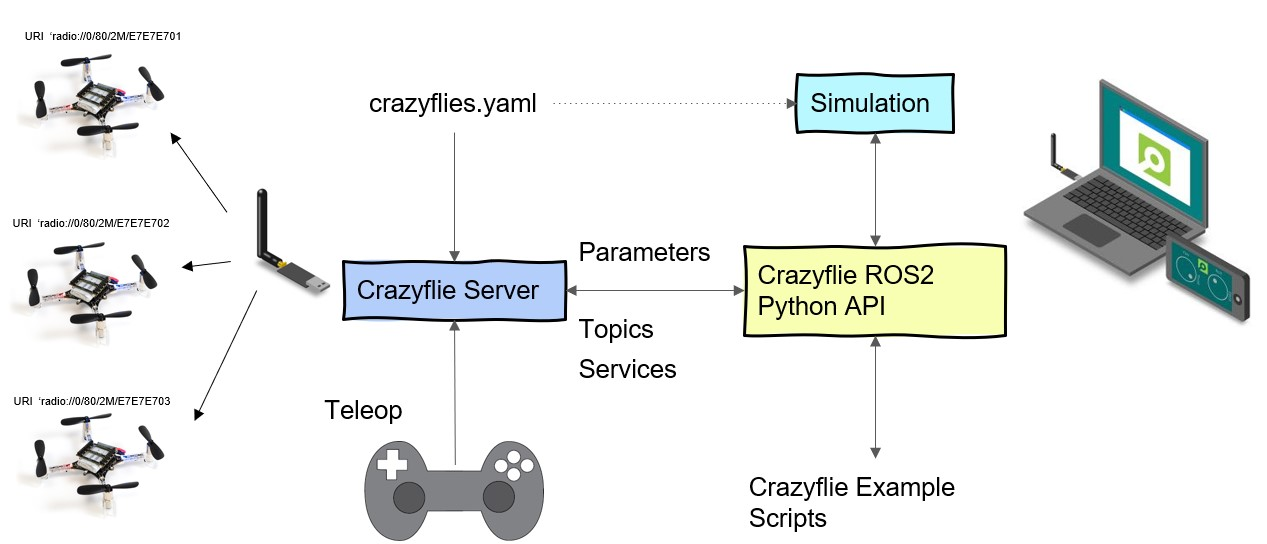
\includegraphics[width=0.5\textwidth]{figuras/overview_nodes.jpg}
    \caption{Estructura de control de Crazyswarm.}
    \cite{Crazyswarm2}
    \label{fig:nodos}
\end{figure}

El protocolo CRTP fue diseñado para permitir una priorización de paquetes y volver más eficiente la comunicación con el drone, permitiendo enviar una trayectoria mientras el drone se controla en tiempo real, siempre que el puerto de la trayectoria sea de mayor prioridad. Cada paquete CRTP contiene un puerto (4 bits), un canal (2 bits), y una carga de hasta 31 bytes. Para crear la conexión del protocolo se debe habilitar el \emph{link} USB usando un paquete de control USB, luego el \emph{link} Radio mantiene dos contadores de paquete para garantizar que no habrá pérdida de paquetes. Finalmente, el subsistema \emph{log} mantiene un estado de todos los bloques \emph{log} y continua enviado información aún si se pierde el \emph{link}\cite{CRTP}

Otro protocolo de comunicación para Crazyflie es el CPX (\emph{Crazyflie Packet eXchange}), el cual fue diseñado para funcionar a bajo nivel y que se empleen otros protocolos por encima. Su función es solucionar el problema de distribuir paquetes a través de múltiples microcontroladores ya que este problema no existía cuando se diseñó el protocolo CRTP, por lo que es un protocolo complementario. Debido a que se utiliza entre microcontroladores, puede enviarse de múltiples formas, como Wi-Fi/TCP, SPI o UART dependiendo de los microcontroladores a comunicar y los módulos adicionales que se implementen en el drone. Este protocolo permite el manejo de paquetes grandes, donde paquetes por debajo de 30 bytes se entregan en un bloque y paquetes más grandes pueden separarse en bloques y un identificador especifica cual es el bloque final.

Para establecer la comunicación de Crazyswarm, el servidor de Crazyflie se conecta con múltiples drones mediante una o más antenas de radiofrecuencia. Se cuenta con dos \emph{backends} a elegir, el ''cpp'' basado en la capa más baja y el ''cflib'', que funciona con Python a un nivel más alto. Este puede manejar aspectos de comunicación de bajo nivel, como recibir los parámetros del Crazyflie y convertirlos a parámetros de ROS2 para crear los parámetros de Crazyflie basado en la entrada.

Crazyflie cuenta con una máquina virtual, la cual funciona mediante Ubuntu y esta contiene todas las librerías para controlar los drones mediante una antena de radiofrecuencia USB. Estas librerías pueden visualizarse y editarse mediante Microsoft Visual Studio, que ya cuenta instalados los compiladores de C++ y Python. Desde Visual Studio, pueden iniciarse los códigos y, si la antena está conectada y un Crazyflie está encendido, pueden realizarse pruebas de movimiento y obtención de datos del drone. La máquina virtual también cuenta con el cliente de Crazyflie, desde el cual puede controlarse al Crazyflie mediante un control externo y es posible visualizar los ángulos de rotación del drone en tiempo real. En caso de que no se cuente con un control externo, puede utilizarse la aplicación para Android de Crazyflie y controlar al drone mediante \emph{Bluetooth}.

\begin{figure}[t]
    \centering
    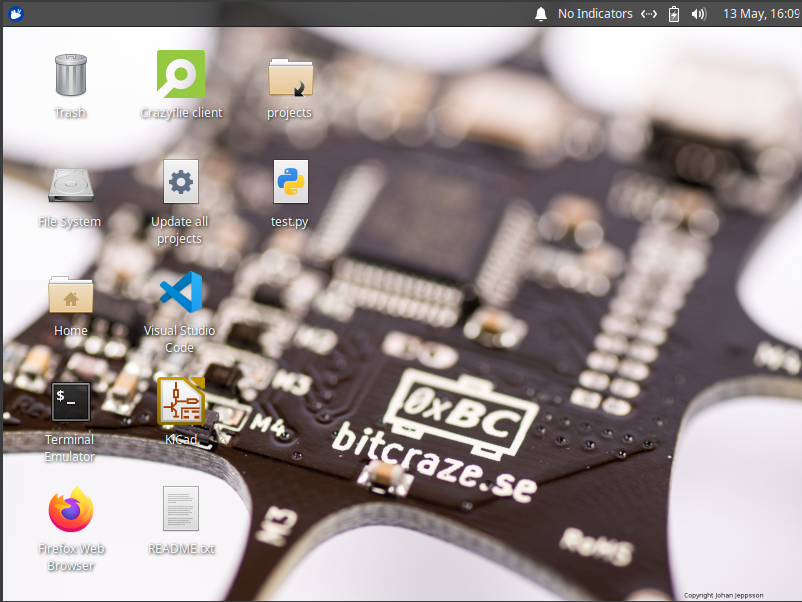
\includegraphics[width=0.5\textwidth]{figuras/VM_Crazyflie.png}
    \caption{Maquina Virtual de Crazyflie.}
    \label{fig:VM}
\end{figure}

Para poder realizar las pruebas del Crazyflie es necesario configurar el puerto de la antena durante la instalación de la máquina virtual, lo cual puede realizarse fácilmente mediante Oracle. También se deben configurar todos los dispositivos que se planeen utilizar en la máquina virtual, de lo contrario no serán reconocidos. Una vez instalada la máquina virtual se debe abrir una terminal e instalar ciertas librerías mediante el gestor de paquetes pip3. Las librerías son:
\begin{itemize}
    \item Matplotlib.
    \item Pandas.
    \item Canvas.
    \item pyinstaller.
\end{itemize}

Finalmente, es necesario actualizar las librerías de los controladores. Esto se logra mediante la opción incluída en el escrictorio de la máquina virtual, como se ve en la Figura 4 \ref{fig:VM}. Sin embargo, se presenta un problema al actualizar las librerías ya que luego de hacerlo deja de funcionar el cliente para controlar el drone con un control externo, por lo que si se desea trabajar con las librerías de Python y con el cliente se recomienda instalar dos máquinas virtuales y que una de estas no se actualice. 


	\fi
\fi

% CAPÍTULOS
% ------------------------------------------------------------------------------
\newpage
\ifdefined\parpordefecto
	\defaultparformat{j-capitulos}
\else
	\chapter{Derivación de la dinámica del mecanismo}

\section{Dinámica de cuerpos rígidos}

\section{Restricciones}
\subsection{Mecanismos de lazo cerrado}
\subsubsection{Mecanismo de cuatro barras}

\chapter{Control del sistema mecánico}

\section{La ecuación del manipulador}

\begin{table}[h]
\begin{tabular}{|l|l|l|l|l|}
\hline
12       & $3.2$  & $3.43$    & 23    & 13      \\ \hline
aasdasdd & asd & ssdssa & ssdas & asdasda \\ \hline
         &     &        &       &         \\ \hline
         &     &        &       &         \\ \hline
\end{tabular}
\caption[Tabla de prueba]{Tabla de prueba. Esta es una breve descripción de la tabla anterior. Continuamos con la descripción de esta forma y se menciona que fue de elaboración propia.} 
\label{cuadro:tablaprueba}
\end{table}

Aquí seguimos escribiendo texto normalmente.
\fi

% CONCLUSIONES
% ------------------------------------------------------------------------------
\ifdefined\CAPconclusiones
	\newpage
	\chapter{Conclusiones}
	\ifdefined\parpordefecto
		\defaultparformat{k-conclusiones}
	\else
		\input{k-conclusiones}
	\fi
\fi

% RECOMENDACIONES
% ------------------------------------------------------------------------------
\ifdefined\CAPrecomendaciones
	\newpage
	\chapter{Recomendaciones}
	\ifdefined\parpordefecto
		\defaultparformat{l-recomendaciones}
	\else
		\input{l-recomendaciones}
	\fi
\fi

% BIBLIOGRAFÍA
% ------------------------------------------------------------------------------
\ifdefined\CAPbibliografia
	\newpage
    \cleardoublepage\phantomsection
	\chapter{\bibname}
    \printbibliography[heading=none]
\fi

% ANEXOS
% ------------------------------------------------------------------------------
\ifdefined\CAPanexos
	\newpage
	\chapter{Anexos}
	\ifdefined\parpordefecto
		\defaultparformat{n-anexos}
	\else
		\section{Planos de construcción}
	\fi
\fi

% GLOSARIO
% ------------------------------------------------------------------------------
\ifdefined\CAPglosario
	\newpage
	\printglossary
\fi

\end{document}